\documentclass{article} % For LaTeX2e
\usepackage{iclr2027_conference,times}

% Optional math commands from https://github.com/goodfeli/dlbook_notation.
\input{math_commands.tex}

\usepackage{hyperref}
\usepackage{url}
\usepackage{booktabs}
\usepackage{graphicx}
\usepackage{amsmath}
\usepackage{amssymb}
\usepackage{xcolor}
\usepackage{multirow}

\newcommand{\fix}{\marginpar{FIX}}
\newcommand{\new}{\marginpar{NEW}}

\title{Never Formed or Later Lost? Measuring Correct-Answer Information Dynamics in Large Language Models}

% Authors hidden for anonymous submission
\author{Anonymous Author(s) \\
Affiliation \\
Address \\
\texttt{email}
}

%\iclrfinalcopy % Uncomment for camera-ready version, but NOT for submission.
\begin{document}

\maketitle

\begin{abstract}
A large language model (LLM) can give a wrong answer for two very different internal reasons: the correct answer never became a competitive candidate inside the model, or it briefly became competitive at an intermediate layer and then lost that advantage by the final layer. These two cases produce the same observable output but represent distinct failure patterns that suggest different intervention strategies. We trace the correct-answer signal layer by layer across Transformer architectures, introducing a calibrated procedure to separate these failure modes. For each question, we construct a layered trajectory of the correct answer's probability, full-vocabulary rank, and margin over competing tokens across three model families (Qwen, Llama, Mistral, 4B to 14B parameters) and three tasks (TriviaQA, HotpotQA, GSM8K). We first show that a common evaluation shortcut, checking whether the intermediate correct answer's logits ever exceed the final wrong output, is misleading: such sign flips occur in over 90\% of errors, but a random-competitor null produces an even higher rate (99\%), showing that pairwise crossings are a trivially weak criterion rather than evidence of prior competitiveness. After correcting for this selection bias and readout miscalibration, we find that most errors are \emph{formation failures} (where the correct signal never forms), and only a small, task-dependent subset represents a \emph{preservation failure} (where the signal forms but later decays). Furthermore, these layer trajectories are predictive: features from the first half of the network predict subsequent signal decay (AUC 0.75under cross-validation;0.66 using only endpoint-free gold-token features), substantially outperforming single-layer confidence baselines, and this predictive structure transfers across tasks and model families. To facilitate research on process-level error diagnosis, we construct and release \texttt{InfoDyn-Bench}, a benchmark containing layered information trajectories, metrics, and prediction labels.
\end{abstract}

\section{Introduction}

When a language model produces a wrong answer, the final output does not reveal how the failure happened \citep{ji2023survey, huang2023survey}. The correct answer may never have become a competitive candidate within the model, or it may have emerged at an intermediate layer and then been weakened by later computation. Both paths end at the same wrong string, yet they represent distinct internal failures that suggest fundamentally different responses: a formation failure indicates insufficient model capability that requires additional training or retrieval augmentation, whereas a preservation failure indicates that the model possessed the relevant signal but lost it during late-layer computation, making it amenable to lightweight inference-time intervention. Distinguishing these two cases is therefore not merely a diagnostic curiosity but a practical deployment decision: across five tasks, we find that the proportion of errors amenable to intervention varies from 5\% (math reasoning) to 29\% (knowledge QA), and that selectively intervening only on predicted preservation failures improves per-intervention efficiency by 127\% while saving 72\% of the intervention budget compared to indiscriminate intervention.

However, making this distinction reliably is surprisingly difficult. From the model's output alone, the two failure types are indistinguishable. Prior work has attempted to identify preservation-like behavior by checking whether the correct answer ever outranks the final wrong output at an intermediate layer, but we show this criterion is trivially satisfied (99\% of errors pass a random-competitor null), rendering it useless for distinguishing genuine signal formation from noise.

\begin{figure}[t]
\centering
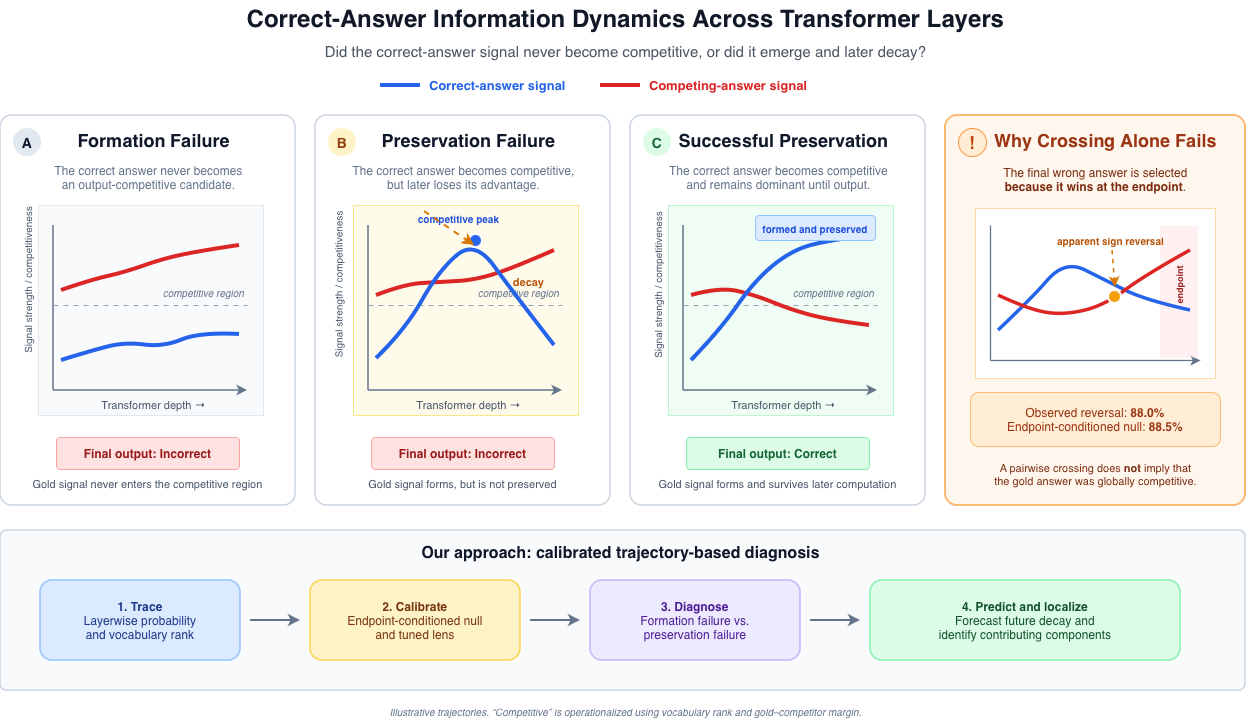
\includegraphics[width=0.95\textwidth]{figures/fig1_concept.pdf}
\caption{Conceptual overview of Information Dynamics. When an LLM outputs an incorrect answer, internal representations may either fail to form a competitive gold-answer signal (\emph{formation failure}) or build a competitive signal at intermediate layers that decays before the final layer (\emph{preservation failure}). Our calibrated framework traces these dynamics across layers.}
\label{fig:concept}
\end{figure}

We distinguish two internal scenarios, as illustrated in Figure~\ref{fig:concept}. Operationally, we define a correct-answer signal as \emph{competitive} at a given layer if the ground-truth answer token $y^\star$ (the \emph{gold answer}) enters the top region of the vocabulary distribution (e.g., top-5 rank) and holds a positive probability margin over competing tokens. Under this criterion, a \emph{formation failure} occurs when the gold answer never achieves competitiveness at any intermediate layer. A \emph{preservation failure} occurs when the gold answer becomes competitive at an intermediate layer but subsequently decays, losing its advantage by the final output layer.

Recognizing these two cases is harder than it looks. A common shortcut decodes intermediate hidden states (e.g., via logit lens \citep{nostalgebraist2020logitlens}) and checks whether the gold answer ever outranks the final wrong answer. We show this shortcut is fundamentally misleading for two key reasons. First, pairwise crossing is a trivially weak criterion: a random-competitor null (replacing the actual final competitor with a randomly selected token) produces an even higher crossing rate (99\% vs. 92\% observed), showing that almost any token will be temporarily outranked by gold at some layer regardless of whether the gold signal was ever truly competitive. Second, directly applying the final layer's output head to intermediate states misreads the signal, because early hidden states occupy a different vector space than the output layer \citep{belrose2023tunedlens, din2023jump}. An uncorrected pairwise logit lead therefore offers no evidence that a competitive signal ever formed.

To reliably diagnose model errors, we introduce \emph{Information Dynamics}, a framework that tracks how the correct answer evolves layer by layer. For each input, we construct a layered trajectory measuring three vocabulary-wide metrics at every layer: the gold answer's log-probability, its full-vocabulary rank, and its margin over top competing candidates. We pair these trajectories with two calibration controls: a randomized null baseline to rule out chance flips caused by final-output selection bias, and a per-layer linear translator (\emph{tuned lens} \citep{belrose2023tunedlens}) to decode intermediate hidden states fairly into vocabulary probabilities. Across six LLMs (4B to 14B parameters) and three tasks, our framework reveals that most errors are formation failures, whereas preservation failures constitute a small, task-dependent subset, concentrated in knowledge QA. Crucially, these trajectories are not merely descriptive but predictive: early-layer trajectory prefixes predict subsequent signal decay (AUC 0.79), substantially outperforming single-layer confidence baselines, and this predictive structure transfers across tasks and model families.

In summary, our paper advances error diagnosis through five key contributions:
\begin{enumerate}
    \item \textbf{Shortcut Invalidation:} We demonstrate that uncorrected pairwise sign flips cannot establish prior signal competitiveness: a random-competitor null produces even higher crossing rates, showing that ``ever crossing'' is a trivially weak criterion.
    \item \textbf{Calibrated Failure Taxonomy:} We propose a calibrated taxonomy separating formation from preservation failures, showing that preservation failures are a task-dependent minority concentrated in knowledge-intensive and science-reasoning tasks.
    \item \textbf{Predictive Trajectory Dynamics:} We establish that early trajectory history carries dynamic predictive signals that forecast future decay better than single-layer confidence snapshot baselines, with cross-task and cross-model transfer.
    \item \textbf{Actionable Diagnosis:} We show that the trajectory-based taxonomy provides a non-oracle intervention trigger: selectively steering only predicted preservation failures improves per-intervention efficiency by 127\% while preservation failures recover at 3.7$\times$ the rate of formation failures under identical non-oracle steering.
    \item \textbf{Benchmark Resource:} We release \texttt{InfoDyn-Bench}, a benchmark of layered information trajectories, derived dynamics metrics, and failure labels across six models and five tasks, to support process-level LLM error analysis.
\end{enumerate}

\section{Related Work}

\subsection{Decoding Intermediate Representations}
Logit lens \citep{nostalgebraist2020logitlens} and tuned lens \citep{belrose2023tunedlens} decode intermediate hidden states back into the vocabulary space. Probing studies ask whether linguistic or factual information is decodable at specific layers using diagnostic classifiers \citep{alain2016understanding, tenney2019bert, hewitt2019structural, belinkov2022probing}. Short-circuiting and early exit approaches study early prediction readiness \citep{schuster2022confident, din2023jump}. These works ask whether a signal is \emph{present} at a given layer. We instead study how a correct-answer signal \emph{evolves dynamically across layers} and systematically quantify readout and selection biases.

\subsection{Knowledge and Factual Recall}
Work on factual knowledge localization, knowledge neurons, and model editing asks where factual associations are stored in feed-forward layers \citep{geva2021transformer, dai2022knowledge, meng2022rome, meng2023memit, geva2023dissecting}. Known-versus-unknown detection and latent knowledge discovery investigate whether internal representations track model correctness \citep{kadavath2022language, burns2022discovering, azaria2023internal, yin2023do, li2024inference}. We do not aim to edit or locate static facts; instead, we track how the correct-answer signal dynamically rises or decays along the network's depth dimension.

\subsection{Hallucination and Error Prediction}
Uncertainty estimation, hidden-state failure prediction, and hallucination detection analyze intermediate representations to identify potential errors \citep{schuster2022confident, kuhn2023semantic, azaria2023internal, manakul2023selfcheckgpt}. Most directly related to our work, \citet{jiang2024hallucination} study layer-wise inference dynamics of correct versus hallucinated outputs using residual-stream decoding and report that dynamic probability curves can predict hallucination. \citet{kim2025uncertainty} extend this to uncertainty-aware layer-wise analysis across multiple models and datasets. Our work differs in three concrete ways: (i)~we demonstrate that naive pairwise logit crossings are explained by an endpoint-conditioned selection bias, establishing a calibration step that prior layer-wise analyses do not include; (ii)~we distinguish formation failures from preservation failures as an operational taxonomy rather than treating all layer-wise dynamics as a single phenomenon; and (iii)~we evaluate whether early-trajectory features carry predictive information \emph{beyond} simple temporal extrapolation (AR baselines, final-layer confidence), whereas prior work predicts error versus correct output categories without ablating temporal autocorrelation.

\subsection{Mechanistic Interpretability and Causal Intervention}
Transformer circuit analysis, direct logit attribution, and activation patching decompose network computations into functional components \citep{elhage2021mathematical, olsson2022incontext, wang2022interpretability, nanda2023progress}. Representation engineering and activation steering modify hidden states to alter output behavior \citep{turner2023activation, rimsky2023steering, zou2023representation}. We perform component-level attribution on information trajectories to isolate the late-layer components associated with correct-signal decay, complementing rather than relying on a particular steering method.

To our knowledge, no prior work combines selection-bias calibration of intermediate readouts with an operational formation-versus-preservation failure taxonomy and demonstrates that trajectory shape predicts future decay beyond temporal-extrapolation baselines.

\section{Problem Definition}
\label{sec:def}

We fix notation here so that every symbol is defined once.

\subsection{Setup}
Let $x$ be a question, $y^\star$ the gold-answer token, and $\hat{y}$ the token the model actually generates. Let $L$ be the number of layers. At layer $\ell$ ($1 \le \ell \le L$), let $h_\ell(x) \in \mathbb{R}^d$ be the hidden representation at the target position, where $d$ is the hidden dimension. Let $W_U \in \mathbb{R}^{d \times |V|}$ denote the unembedding matrix, where $|V|$ is the vocabulary size, and let $w_y \in \mathbb{R}^d$ be the unembedding vector corresponding to token $y$. A lens $g_\ell$ maps the representation to a logit vector, which we turn into a distribution over the vocabulary by a softmax:
\begin{equation}
p_\ell(y \mid x) = \operatorname{softmax}(g_\ell(h_\ell(x)))_y .
\end{equation}
We use two lenses. The raw logit lens \citep{nostalgebraist2020logitlens} sets $g_\ell$ to the final language-model head, applying the final layer norm and unembedding matrix $W_U$. The tuned lens \citep{belrose2023tunedlens} adds a per-layer affine map that is trained so that the decoded logits approximate the final-layer logits.

We define the \emph{gold rank} $r_\ell(y^\star)$ as the number of tokens whose probability at layer $\ell$ strictly exceeds that of the gold answer. With this zero-based convention, $r_\ell(y^\star) = 0$ means the gold answer is the top-1 token at layer $\ell$, and the competitiveness test $r_\ell(y^\star) \le k$ used below means that at most $k$ tokens outrank the gold answer:
\begin{equation}
r_\ell(y^\star) = \sum_{y \neq y^\star} \mathbb{1}\big[ p_\ell(y) > p_\ell(y^\star) \big] .
\end{equation}
All reported ranks use this zero-based convention.

\subsection{Two Competitive Margins}
We use two related margins in different analyses. The first compares the gold answer with the generated answer $\hat{y}$:
\begin{equation}
\mathrm{CIS}^{\mathrm{gen}}_\ell = \log p_\ell(y^\star) - \log p_\ell(\hat{y}), \qquad \hat{y} \neq y^\star .
\end{equation}
We use this margin for error examples and for the endpoint-bias analysis. The second compares the gold answer with the strongest competing token $y^-$, defined as the most probable token other than the gold answer at the final layer:
\begin{equation}
y^- = \arg\max_{y \neq y^\star} p_L(y), \qquad
\mathrm{CIS}^{\mathrm{comp}}_\ell = \log p_\ell(y^\star) - \log p_\ell(y^-) .
\end{equation}
We fix $y^-$ at the final layer and track it across all layers rather than re-selecting the strongest competitor at each layer independently. This design choice ensures that the margin measures a consistent quantity across depths: it tracks whether the gold answer gains or loses ground against a fixed reference competitor, making the trajectory comparable across layers. A per-layer competitor $\arg\max_{y \neq y^\star} p_\ell(y)$ would make each layer's margin measure a different comparison and would reduce $\mathrm{CIS}^{\mathrm{comp}}_\ell > 0$ to the condition $r_\ell(y^\star) = 0$ (gold is rank-1), which is too strict. Our joint criterion requires both vocabulary-wide competitiveness ($r_\ell \le k$, ensuring the gold answer is broadly competitive) and a positive margin against the eventual output competitor ($\mathrm{CIS}^{\mathrm{comp}}_\ell > 0$, ensuring it leads the token it will ultimately lose to). We use this margin whenever we compare correct and incorrect examples. Table~\ref{tab:metric} states which margin each analysis uses, so the measurement object is never ambiguous.

\begin{table}[t]
\centering
\caption{Which margin each analysis uses.}
\label{tab:metric}
\begin{tabular}{ll}
\toprule
\textbf{Analysis} & \textbf{Margin} \\
\midrule
Endpoint selection bias & $\mathrm{CIS}^{\mathrm{gen}}$ \\
Correct versus incorrect comparison & $\mathrm{CIS}^{\mathrm{comp}}$ \\
Competitive-decay classification & $\mathrm{CIS}^{\mathrm{comp}}$ \\
Trajectory prediction & $\mathrm{CIS}^{\mathrm{comp}}$ \\
Direct logit attribution & $\mathrm{CIS}^{\mathrm{comp}}$ \\
\bottomrule
\end{tabular}
\end{table}

\subsection{Information Trajectory}
The information trajectory of an example is the per-layer collection of the gold log-probability, the gold rank, and the competitive margin:
\begin{equation}
\mathcal{T}(x) = \big\{ \log p_\ell(y^\star),\; r_\ell(y^\star),\; \mathrm{CIS}^{\mathrm{comp}}_\ell \big\}_{\ell=1}^{L} .
\end{equation}
From this trajectory we derive three quantities. The \emph{peak rank} is the smallest rank over all layers except the final one:
\begin{equation}
r_{\mathrm{peak}} = \min_{1 \le \ell < L} r_\ell(y^\star) .
\end{equation}
The \emph{peak-to-final decay} $D$ is the drop from the largest intermediate margin to the final margin:
\begin{equation}
D = \max_{1 \le \ell < L} \mathrm{CIS}^{\mathrm{comp}}_\ell \;-\; \mathrm{CIS}^{\mathrm{comp}}_L .
\end{equation}
The \emph{competitive decay} label marks an example whose gold answer is competitive at some intermediate layer but negative at the final layer:
\begin{equation}
C(x) = \mathbb{1}\Big[ \exists\, \ell < L : r_\ell(y^\star) \le k \;\land\; \mathrm{CIS}^{\mathrm{comp}}_\ell > 0 \Big] \cdot \mathbb{1}\Big[ \mathrm{CIS}^{\mathrm{comp}}_L < 0 \Big] .
\end{equation}
We use $k=5$ as the main competitiveness threshold and report the sensitivity over $k \in \{1,5,10,50\}$ (Section~\ref{sec:taskdecay}).

The top-$k$ criterion is not an arbitrary empirical cut: it marks a robust transition in output-space decodability. At the first layer where the gold token's rank drops to $\le k$, the gold log-probability jumps by about $+8$ logit units, from a noise-level value (median $\approx -11$, a probability of $\sim 10^{-5}$) to a substantive value (median $\approx -2.7$, a probability of $\sim 0.07$ at $k=5$); this jump is positive in $97\%$ of samples and remains large for every $k \in \{1,5,10\}$ (medians $+7.6$, $+8.0$, $+7.5$). Entering the top-$k$ therefore corresponds to the moment the gold answer emerges from vocabulary noise into a decodable candidate, which is why the competitiveness threshold, within a reasonable range, tracks a consistent output-readiness transition rather than an arbitrary decision boundary.

\subsection{Error Taxonomy}
We define four operational categories under our measurement framework. They describe what the measurement sees, not every conceivable error mechanism. A \emph{formation failure} is an incorrect example whose gold answer never meets the competitiveness criterion at any intermediate layer. A \emph{preservation failure} is an incorrect example whose gold answer meets the criterion but loses its advantage by the final layer. A \emph{successful preservation} is a correct example whose signal forms and is maintained. The remaining category, \emph{unresolved}, covers examples where tracking only the final-answer token is not enough to describe the error, such as multi-step reasoning.

\section{Experimental Setup}

\subsection{Models and Tasks}
We evaluate three open-weight instruction-tuned model families spanning several scales: Qwen3-14B, Qwen3-8B, Qwen3-4B, and Qwen2.5-7B for scale variation within Qwen, plus Llama-3.1-8B \citep{dubey2024llama} and Mistral-7B-Instruct-v0.3 \citep{jiang2023mistral}. We use three tasks: TriviaQA \citep{joshi2017triviaqa} for fact QA, HotpotQA \citep{yang2018hotpotqa} for multi-hop QA, and GSM8K \citep{cobbe2021gsm8k} for math reasoning.

\subsection{Answer Extraction}
We judge correctness by exact substring matching after lower-casing. For numeric answers we strip commas and percent signs and compare numerically with a small tolerance. For TriviaQA, where several aliases are valid, a match against any alias counts as correct.

\subsection{Lens Construction}
The raw logit lens applies the final language-model head directly. For the tuned lens \citep{belrose2023tunedlens} we fit, for each layer, an affine map $(\mathbf{A}_\ell, \mathbf{b}_\ell)$ so that $\mathbf{A}_\ell h_\ell + \mathbf{b}_\ell$, decoded through the final norm and head, approximates the final-layer logits. Each layer's translator is trained independently on a held-out prompt subset, minimizing the mean-squared error between the decoded logits and the model's own final-layer logits (Adam, learning rate $10^{-3}$, $500$ epochs). Because the objective is supervised by the model's own final logits rather than by the answer label, the translators never see the gold answer or the correctness label, so no ground-truth answer labels leak through the lens (although the lens does learn to approximate the final output distribution).

\subsection{Statistical Testing}
We report every proportion with a bootstrap 95\% confidence interval, and we report per-model and per-task numbers alongside aggregates.

\section{Results}

\subsection{Pairwise Sign Flips Fail to Establish Intermediate Signal Competitiveness}

\paragraph{Testing the shortcut against null baselines.}
We first evaluate the common shortcut of checking whether the gold answer's intermediate probability ever exceeds that of the final incorrect prediction. Across error examples, we observe that the gold token's log-probability surpasses the final competitor at some intermediate layer in 92\% of cases. To assess whether this is meaningful, we construct a random-competitor null: for each error, we replace the true final competitor with the generated token from a different, randomly selected error example, and recompute the crossing rate. Under this null the crossing rate is even higher (99\%), because a randomly chosen competitor is typically weaker than the model's actual final prediction. The fact that the observed crossing rate is \emph{lower} than this null, rather than being inflated, shows that the "ever crossing" statistic is simply too weak a criterion: almost any token will be crossed by gold at some layer, regardless of whether the gold signal was ever truly competitive. Pairwise logit crossings therefore offer no empirical evidence that a gold signal was ever meaningfully formed.

\paragraph{Why shortcut analysis misleads.}
Pairwise comparison fails because beating a single wrong output token does not imply that the gold answer achieves a high rank within the overall vocabulary. Furthermore, directly projecting intermediate states through the final language-model head inflates peak intermediate margins by approximately 2.0$\times$ relative to calibrated readouts (median peak margin 4.53 vs. 2.24 logit units on Qwen3-8B; Figure~\ref{fig:bias}, right). We therefore abandon pairwise sign-flip heuristics and adopt the vocabulary-wide rank and margin criterion defined in Section~\ref{sec:def}.

\begin{figure}[t]
\centering

\includegraphics[width=0.85\textwidth]{figures/fig2_measurement_bias.pdf}
\caption{Measurement bias in intermediate state decoding. Left: observed pairwise crossing rate (92\%) is lower than a random-competitor null (99\%), showing that crossing is a trivially weak criterion. Right: the uncalibrated raw logit lens inflates intermediate peak margins by ~2.0$\times$ relative to the tuned lens.}
\label{fig:bias}
\end{figure}

\subsection{Correct and Incorrect Outputs Follow Distinct Information Trajectories}

\paragraph{Persistent signal formation in correct predictions.}
Across all evaluated architectures and scales, correct predictions establish a strong, persistent gold-answer signal early in the network, whereas incorrect predictions show weak initial formation and substantial late-layer decay (Figure~\ref{fig:trajectories}). As reported in Table~\ref{tab:rank}, median intermediate peak ranks for correct outputs reach top positions across models (0 for Qwen3-8B, 1 for Llama-3.1-8B, 1 for Qwen3-14B), with 90.5\% of correct Qwen3-8B examples entering the top-5 candidate set. In contrast, incorrect outputs exhibit significantly worse peak ranks (median 19 for Qwen3-8B, 20 for Llama-3.1-8B, 77 for Mistral-7B) and lower top-5 entry rates (26.4\% for Qwen3-8B).

\begin{table}[t]
\centering
\caption{Median peak rank (excluding the final layer) and top-5 entry rate for correct versus incorrect predictions across model families and scales.}
\label{tab:rank}
\begin{tabular}{lcccc}
\toprule
\textbf{Model} & \multicolumn{2}{c}{\textbf{Correct Predictions}} & \multicolumn{2}{c}{\textbf{Incorrect Predictions}} \\
\cmidrule(lr){2-3}\cmidrule(lr){4-5}
 & Peak Rank & Top-5 Entry & Peak Rank & Top-5 Entry \\
\midrule
Qwen3-14B & 1 & \cdot & 9 & \cdot \\
Qwen3-8B & 0 & 90.5\% & 19 & 26.4\% \\
Qwen3-4B & 2 & \cdot & 10 & \cdot \\
Qwen2.5-7B & 1 & \cdot & 26 & \cdot \\
Llama-3.1-8B & 1 & 79.6\% & 20 & 26.7\% \\
Mistral-7B & 11 & 30.2\% & 77 & 8.4\% \\
\bottomrule
\end{tabular}
\end{table}

\paragraph{Probe robustness across independent decoders.}
To confirm that this intermediate rank separation is a genuine property of the internal representations rather than an artifact of the raw logit lens, we recomputed peak intermediate ranks under three independent decoding methods: the raw logit lens, the tuned lens, and a parameter-free cosine similarity between intermediate hidden states $h_\ell$ and unembedding vectors $w_{y^\star}$. Across all three decoders, correct and incorrect predictions remain separated by over an order of magnitude in rank (medians 0 vs. 32 for raw lens, 0 vs. 12 for tuned lens, 1 vs. 43 for training-free cosine similarity; Mann-Whitney $p < 10^{-20}$ in all cases). Because cosine similarity uses no learned parameters or final layer normalization, the separation is robust across multiple readout methods and is not an artifact of any single decoder.

\begin{figure}[t]
\centering
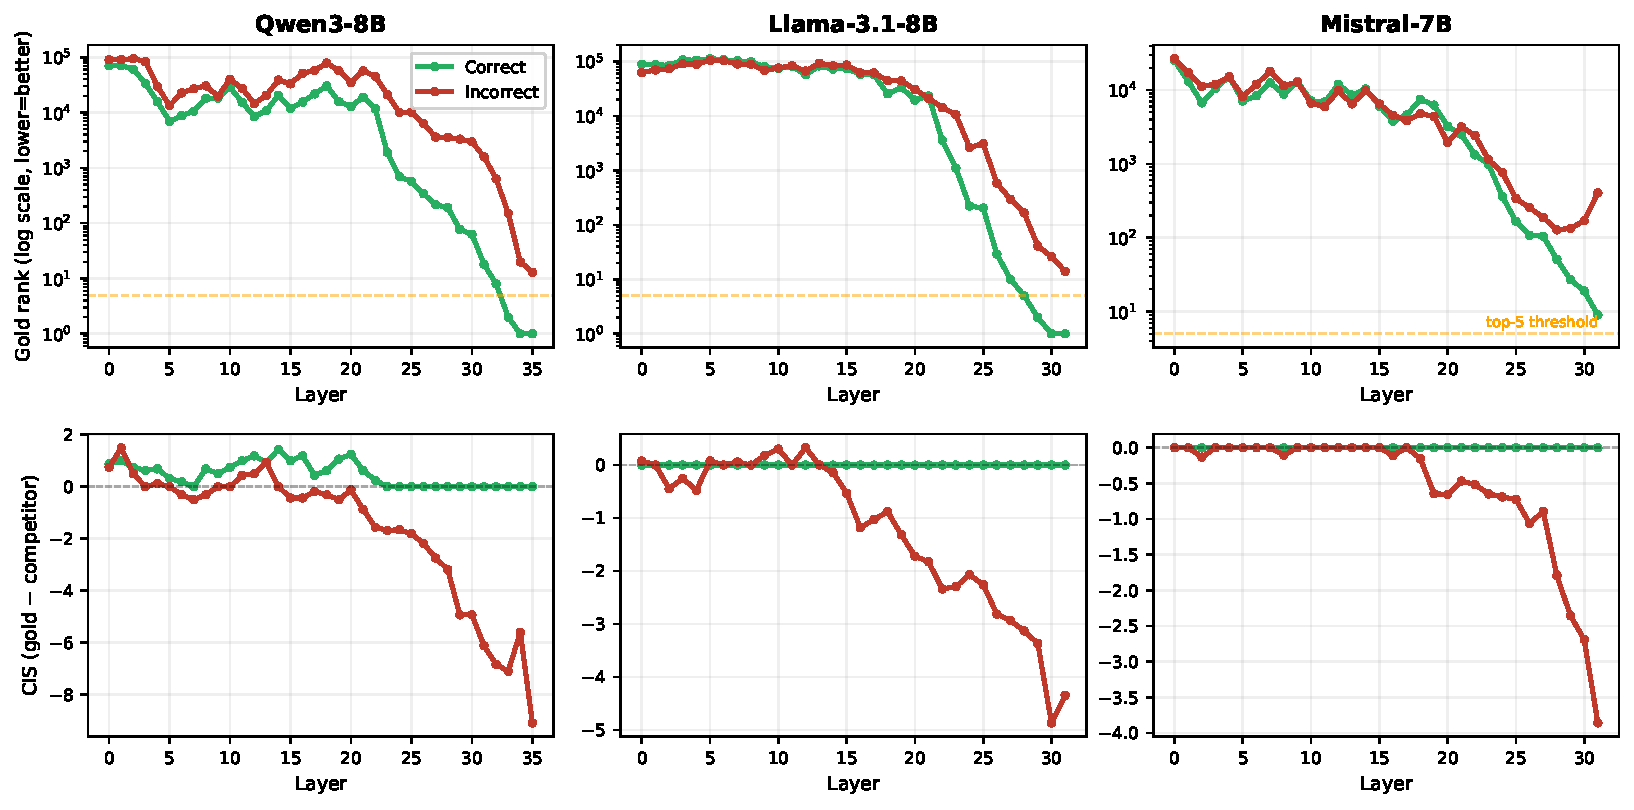
\includegraphics[width=0.95\textwidth]{figures/fig3_trajectories.pdf}
\caption{Median gold-answer rank (top, log scale) and probability margin (bottom) across layers for correct (green) and incorrect (red) predictions across model families.}
\label{fig:trajectories}
\end{figure}

\subsection{Calibrated Readout Confirms Preservation Failures Are a Small Minority}

\paragraph{Preservation failure rate under calibrated readout.}
Applying our rank-and-margin criterion ($k=5, \mathrm{CIS}^{\mathrm{comp}}_\ell > 0$) to error examples reveals that preservation failures represent a small minority of total errors. On the Qwen3-8B analysis subset (a balanced sample of the errors, evaluated under the calibrated tuned lens), the uncalibrated raw lens detects a competitive decay rate of 5.2\%, while the calibrated tuned lens identifies 8.9\% (bootstrap 95\% CI [6.4\%, 11.5\%]). Readout calibration slightly increases the detected rate because the tuned lens recovers gold-answer tokens that were geometrically masked under raw projection. Over 91\% of errors are formation failures, where the gold answer never becomes competitive at any intermediate layer. This subset estimate is the figure we report as the headline preservation-failure rate; the per-task rates in Table~\ref{tab:taskdecay} use the full task errors and hence differ slightly in denominator.

\paragraph{Zero label-leakage calibration.}
Crucially, this 8.9\% preservation-failure rate is not a probe artifact. Because our tuned lens translators are trained strictly on unlabelled general prompts by predicting the model's own final-layer logits without observing ground-truth answers or correctness labels, no downstream task information leaks into intermediate readouts. This supports an interpretation where the gold-answer signal becomes decodable at intermediate layers and then loses its competitiveness by the output, rather than being an artifact of uncalibrated projection.

\subsection{Failure Taxonomy Is Task-Dependent and Robust to Thresholds}
\label{sec:taskdecay}

\paragraph{Task dependence: Preservation failures vary widely across reasoning scenarios.}
As detailed in Table~\ref{tab:taskdecay}, preservation failures are highly task-dependent, spanning a wide range from 5\% to 45\% across seven tasks. Long-context reading comprehension (QuALITY) shows the highest rate at 45.2\%, suggesting that correct signals formed during context processing are particularly vulnerable to being overwritten by subsequent computation in deep networks. World knowledge (MMLU) and single-hop factual recall (TriviaQA) follow at 35.9\% and 28.5\%. Science and multi-hop reasoning (ARC-Challenge, HotpotQA) show intermediate rates around 24--25\%. Commonsense reasoning (CommonsenseQA) is markedly lower at 11.8\%, and mathematical reasoning (GSM8K) is lowest at 5.2\%. This gradient reveals a clear pattern: tasks requiring factual retrieval or long-context integration exhibit the highest preservation-failure rates, while tasks requiring multi-step procedural computation exhibit the lowest, consistent with our interpretation that preservation failures arise when the model forms a correct factual association but fails to maintain it through late-layer computation.

\begin{table}[t]
\centering
\caption{Signal-loss rate (preservation failure) by task on Qwen3-8B, measured as the fraction of errors where the gold token enters top-5 at some intermediate layer but drops below rank 10 at the final layer. Tasks are ordered by signal-loss rate.}
\label{tab:taskdecay}
\begin{tabular}{lccc}
\toprule
\textbf{Task} & \textbf{Type} & \textbf{Total Errors} & \textbf{Signal-Loss Rate} \\
\midrule
QuALITY & Long-context comprehension & 199 & 45.2\% \\
MMLU & World knowledge (multi-subject) & 167 & 35.9\% \\
TriviaQA & Knowledge QA & 284 & 28.5\% \\
HotpotQA & Multi-hop QA & 190 & 25.3\% \\
ARC-Challenge & Science reasoning & 229 & 23.6\% \\
CommonsenseQA & Commonsense reasoning & 195 & 11.8\% \\
GSM8K & Math reasoning & 232 & 5.2\% \\
\bottomrule
\end{tabular}
\end{table}

\paragraph{Measurement boundaries on multi-step reasoning.}
The absence of preservation failures on GSM8K reflects a clear operational boundary of final-token tracking rather than evidence that math reasoning never exhibits such failures. First, mathematical answers frequently involve multi-token numbers (e.g., "42"), whereas single-token tracking observes only the final token. Second, in multi-step chain-of-thought reasoning, incorrect final answers stem from intermediate reasoning errors, and the final answer token itself may never form in intermediate layers. Under our final-answer-token measurement, preservation failures are therefore observed specifically in entity-level factual recall rather than in procedural reasoning.

\begin{figure}[t]
\centering
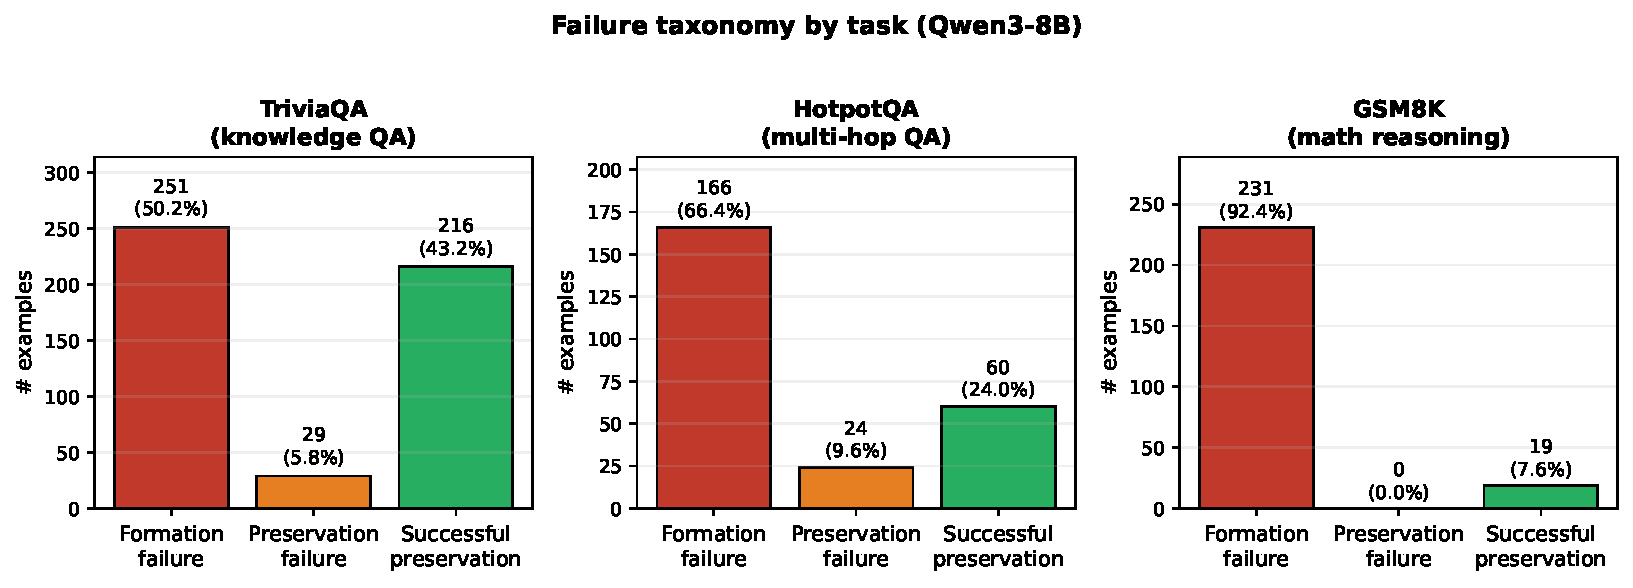
\includegraphics[width=0.95\textwidth]{figures/fig4_taxonomy.pdf}
\caption{Operational error taxonomy across tasks for Qwen3-8B. Preservation failures concentrate in knowledge-intensive QA (TriviaQA, HotpotQA) and are virtually absent in math reasoning (GSM8K).}
\label{fig:taxonomy}
\end{figure}

\paragraph{Robustness across competitiveness thresholds.}
To ensure our taxonomy is not sensitive to the rank cut-off $k$, we re-evaluated the competitive decay rate across $k \in \{1, 5, 10, 50\}$ on Qwen3-8B while holding the margin condition ($\mathrm{CIS}^{\mathrm{comp}}_\ell > 0$) fixed. The preservation-failure rate increases monotonically but slowly: 4.8\% at $k=1$, 8.5\% at $k=5$, 10.1\% at $k=10$, and 16.9\% at $k=50$. Across all reasonable thresholds, preservation failures remain a small minority, confirming the stability of our taxonomy.

\paragraph{Raw versus tuned lens agreement.}
Finally, while the raw logit lens inflates intermediate peak margins by ~2.0$\times$, both lenses yield identical relative trajectory orderings between correct and incorrect predictions. Readout calibration adjusts absolute margin magnitudes without altering the underlying representational dynamics.

\section{Trajectory Dynamics Predict Later Signal Decay}

\paragraph{Predictive validation of the dynamics framework.}
If the information dynamics we measure capture how a model forms and maintains candidate answers, the trajectory prefix should carry predictive signal about future decay. We evaluate this by training a linear classifier on features computed exclusively from the first half of the network ($\ell \le L/2$) to predict a binary second-half decay label. Formally, let $t_0= \lfloor L/2 \rfloor$ be the midpoint layer and define:
\begin{equation}
y^{\mathrm{decay}} = \mathbb{1}\Big[\max_{\ell \in \{t_0,\ldots,L-1\}} \mathrm{CIS}^{\mathrm{comp}}_\ell > 0 \;\;\land\;\; \mathrm{CIS}^{\mathrm{comp}}_L < 0 \Big] .
\end{equation}
That is, the label is positive when the gold signal reaches a positive margin somewhere in the second half of the network but is negative at the final layer. This definition uses only second-half information, so it is strictly separated from the first-half features used for prediction.

\paragraph{Full trajectory dominates single-layer snapshot baselines.}
As shown in Figure~\ref{fig:prediction}a, the full-trajectory model achieves an AUC of 0.79 on Qwen3-8B within-task decay prediction (single held-out split; 5-fold stratified CV gives $0.75 \pm 0.02$, 95\% CI [0.70, 0.80]), substantially outperforming single-layer midpoint snapshot baselines. Common midpoint confidence proxies perform poorly: the gold margin $\mathrm{CIS}_{t_0}$ yields AUC 0.39, midpoint rank yields 0.51, and midpoint output entropy reaches 0.61. Simple summary features such as margin-plus-slope (AUC 0.61) and running maximum (0.61) also fail to capture the full trajectory signal. This demonstrates that historical trajectory evolution adds substantial predictive value beyond any current-state snapshot. We use L2-regularized logistic regression (5-fold stratified CV, StandardScaler normalization, random seed 42); the 5-fold ROC-AUC is $0.75 \pm 0.02$ (95\% CI [0.70, 0.80]) and the out-of-fold average precision (PR-AUC) is 0.71. Because the decay label is positive in 46\% of examples (not a rare event), ROC-AUC and PR-AUC are broadly concordant. Replacing the linear classifier with a random forest (200 trees, max depth 8) raises the 5-fold AUC to $0.92 \pm 0.01$ (permutation test $p < 0.02$), indicating substantial nonlinear predictive structure in the trajectory features; we report the linear result as a conservative lower bound. The nonlinear gain is unlikely to be an artifact of feature engineering: the feature space is only 12-dimensional, regularization via depth limit prevents overfitting, and even a conservative configuration (50 trees, depth 4) reaches 0.91.

\paragraph{Predictive power exceeds final-layer confidence signals.}
We next evaluate whether final-layer output confidence signals can predict decay without intermediate trajectories. We compared first-half trajectory predictions against baselines computed from \emph{final-layer} outputs: final gold margin (AUC 0.67), final gold rank (0.70), and final output entropy (0.68). A baseline combining all three final-layer signals reaches AUC 0.70, whereas the first-half trajectory reaches 0.78. Because the trajectory prefix observes only early hidden states while final-layer baselines observe the fully executed computation, this performance gap confirms that early layer history contains unique dynamic signals that are not captured by final-layer output confidence.

\paragraph{Endpoint conditioning and its scope.}
We note that the competitive margin $\mathrm{CIS}^{\mathrm{comp}}_\ell$ is defined with respect to the final-layer competitor $y^-$, so the first-half features are not purely endpoint-free: the identity of the eventual competitor is determined at the final layer. To quantify the contribution of this endpoint conditioning, we re-trained the predictor using only features that do not reference $y^-$ (the gold log-probability, gold rank, and their slopes, which depend only on the gold token itself). This endpoint-free predictor still achieves AUC 0.66, which remains above all single-layer baselines and temporal-extrapolation baselines (persistence 0.60, AR 0.62), showing that the gold-answer trajectory alone carries predictive signal about future decay. The full trajectory's higher AUC (0.75) reflects additional information from the gold-vs-competitor contrast, which is a legitimate trajectory quantity but does depend on which token ultimately wins. All baselines in our comparison use the same CIS definition, so the relative ordering (full trajectory $>$ AR $>$ persistence) is not affected by this conditioning.

\paragraph{Structure-dependent cross-task generalization.}
As illustrated in Figure~\ref{fig:prediction}b, decay prediction transfers across tasks in a structure-dependent manner. Transfer is strong between entity-style knowledge QA datasets (TriviaQA $\to$ HotpotQA, AUC 0.74) and from multi-hop QA to multi-step math reasoning (HotpotQA $\to$ GSM8K, AUC 0.77). Conversely, transfer from single-step fact recall to multi-step reasoning is weaker (TriviaQA $\to$ GSM8K, AUC 0.38), consistent with our finding that GSM8K final-answer tokens do not form intermediate competitive signals (Section~\ref{sec:taskdecay}). Using a nonlinear classifier (random forest), the strongest cross-task direction (TriviaQA $\to$ HotpotQA) reaches 0.86, confirming that the transferable signal is not saturated by the linear model.

\paragraph{Robust cross-model transfer across architectures.}
To test whether trajectory dynamics reflect shared Transformer properties, we evaluated cross-model transfer across three distinct model families, reporting the results in Table~\ref{tab:crossmodel} and Figure~\ref{fig:prediction}c. Across all model pairs, transfer AUCs consistently exceed chance level, with Qwen3-8B $\to$ Llama-3.1-8B reaching AUC 0.728 and Llama-3.1-8B $\to$ Mistral-7B reaching 0.779. Leave-one-model-out transfer averages AUC 0.739. By aligning layers by relative depth and applying normalization strictly on training models, these results show that the trajectory pattern transfers across the evaluated Transformer families rather than being a single-model fitting artifact.

\begin{table}[t]
\centering
\caption{Cross-model decay-prediction AUC across model families. Rows indicate training models, and columns indicate test models.}
\label{tab:crossmodel}
\begin{tabular}{lccc}
\toprule
\textbf{Train $\backslash$ Test} & Qwen3-8B & Llama-3.1-8B & Mistral-7B \\
\midrule
Qwen3-8B & \cdot & \textbf{0.728} & 0.748 \\
Llama-3.1-8B & 0.695 & \cdot & 0.779 \\
Mistral-7B & 0.639 & 0.599 & \cdot \\
\midrule
Leave-one-out & 0.703 & 0.750 & 0.763 \\
\bottomrule
\end{tabular}
\end{table}

\paragraph{Trajectory decomposition: Dynamic shape drives prediction.}
To isolate which specific dynamic properties drive prediction, we decomposed the trajectory into individual features and evaluated their standalone AUCs (Figure~\ref{fig:trajdecomp}). No single feature matches the full trajectory. The strongest individual dynamic feature is the margin sign oscillation count (transitions, AUC 0.64), followed by peak first-half margin (0.64), first-half variance (0.63), and margin slope (0.61), whereas static midpoint margin (0.60) and rank (0.51) are noticeably weaker. Combining peak, slope, and variance reaches AUC 0.70, while adding full shape features achieves 0.75. This confirms that predictive performance is driven by the joint dynamic evolution of how the signal emerges, peaks, and fluctuates.

\paragraph{The gain is not mere temporal autocorrelation.}
Because the decay label describes the second half of the very trajectory that the first half summarizes, one might suspect the AUC is trivially explained by temporal continuity. To test this, we compared against standard time-series forecasts computed from the first half alone: the last observed value (persistence, AUC 0.60), the first-half linear slope (0.58), linear extrapolation to the final layer (0.58), a first-order autoregressive forecast (0.62), and the first-half mean as a smoothing prior (0.56). All of these lie well below the full trajectory's 0.79. If the predictive signal were just autocorrelation, an autoregressive or extrapolation baseline should approach the full-trajectory model; it does not. The additional predictive power therefore comes from the joint shape of the trajectory, not from simple temporal continuity.

\begin{figure}[t]
\centering

\includegraphics[width=0.95\textwidth]{figures/fig5_prediction.pdf}
\caption{Decay prediction results. (a) Within-task AUC comparing full trajectory against snapshot and final-layer baselines. (b) Cross-task transfer matrix. (c) Cross-model transfer matrix.}
\label{fig:prediction}
\end{figure}

\begin{figure}[t]
\centering
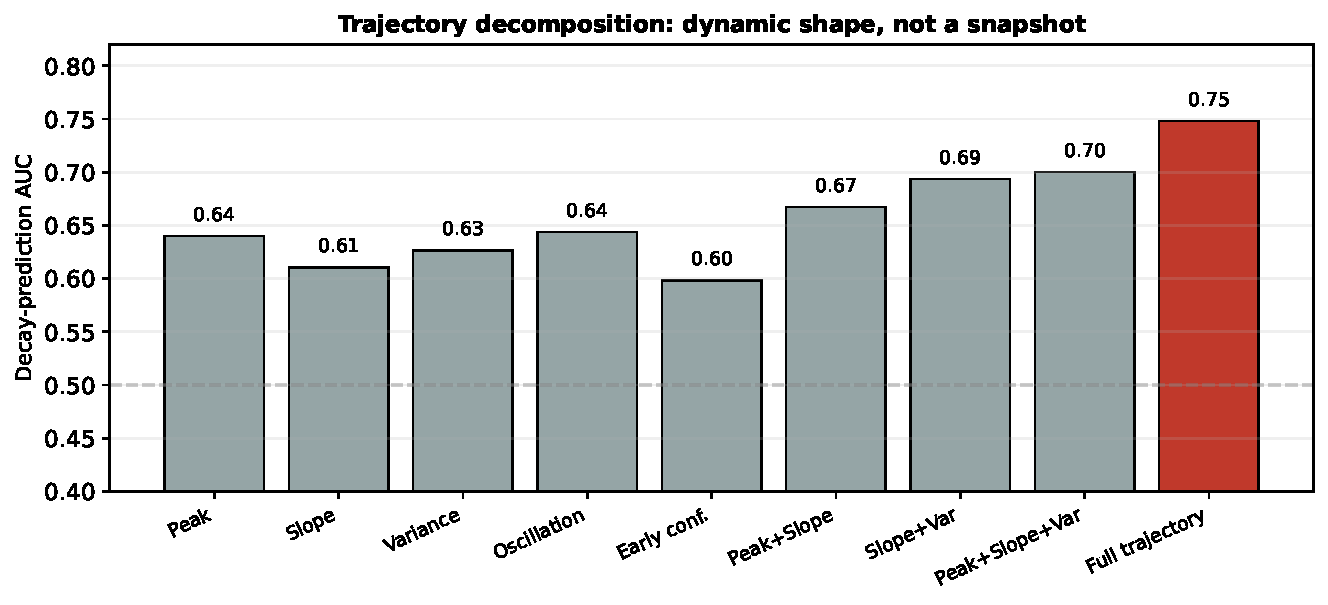
\includegraphics[width=0.95\textwidth]{figures/fig_traj_decomp.pdf}
\caption{Trajectory feature decomposition. Individual dynamic features (peak, slope, variance, transitions) outperform static snapshots, while their combination drives full predictive power.}
\label{fig:trajdecomp}
\end{figure}

\section{Behavioral Intervention and Component Analysis}

\subsection{Gold-Direction Ablation}

We asked whether the correct-answer signal is behaviorally necessary, meaning whether removing it changes the output. We removed the component of the hidden state that lies along the gold token's unembedding direction $w_{y^\star}$ (defined in Section~\ref{sec:def}) in the last three layers:
\begin{equation}
h'_\ell = h_\ell - \operatorname{proj}_{w_{y^\star}}(h_\ell) .
\end{equation}
Here $\operatorname{proj}_{w_{y^\star}}(h_\ell)$ is the projection of $h_\ell$ onto $w_{y^\star}$, so the operation deletes the part of the representation that pushes toward the gold token. We applied this to examples that were originally correct and measured how many flipped to wrong.

The ablation flips correct examples to wrong at high rates across all models, as Table~\ref{tab:ablation} shows.

\begin{table}[t]
\centering
\caption{Behavioral necessity across model families and scales. Ablating the gold direction flips correct examples to wrong at high rates, while a random-token control flips almost none. Parentheses give Wilson 95\% intervals for the gold flip rate.}
\label{tab:ablation}
\begin{tabular}{lcccc}
\toprule
\textbf{Model} & \textbf{Baseline correct} & \textbf{Gold flip} & \textbf{Random token flip} \\
\midrule
Qwen3-14B & 30/30 & 23/30 (77\%, CI [59, 88]) & 0/30 (0\%) \\
Qwen3-8B & 50/50 & 38/50 (76\%, CI [63, 86]) & 0/50 (0\%) \\
Qwen3-4B & 27/27 & 18/27 (67\%, CI [48, 81]) & 0/27 (0\%) \\
Qwen2.5-7B & 30/30 & 26/30 (87\%, CI [70, 95]) & 1/30 (3\%) \\
Llama-3.1-8B & 30/30 & 22/30 (73\%, CI [56, 86]) & 0/30 (0\%) \\
Mistral-7B & 30/30 & 12/30 (40\%, CI [25, 58]) & 0/30 (0\%) \\
\bottomrule
\end{tabular}
\end{table}

The gold flip rates are 77\%, 76\%, 67\%, 87\%, 73\%, and 40\% for Qwen3-14B, Qwen3-8B, Qwen3-4B, Qwen2.5-7B, Llama, and Mistral. The random-token control flips 0\% in almost every model (one example in Qwen2.5-7B). The effect is consistent across model families and across scales from 4B to 14B. The difference between the strongest model (Qwen2.5-7B, 87\%) and the weakest (Mistral-7B, 40\%) is statistically distinguishable: their 95\% intervals, [70, 95] and [25, 58], do not overlap, so the variation across architectures is not merely sampling noise.

\subsection{Controls}

To check that the effect is not just any direction change, we ablated other directions. A key concern is that the gold unembedding direction is the main source of the gold log-probability, so removing it lowers that log-probability more than removing any other direction would. To make the comparison fair, we matched the \emph{perturbation magnitude}: for each control direction, we set the per-layer removal strength so that the hidden-state change $\lVert \Delta h \rVert$ equals that of the gold ablation. This way all interventions change the representation by the same amount and differ only in which direction they remove.

Under this norm-matched protocol, the gold direction flips far more examples than any control, and the gradient is consistent across Qwen scales. On Qwen3-8B, gold flips 83.3\% of correct examples, while the second-best candidate flips 38.9\%, a random token 5.6\%, and a random Gaussian direction 11.1\%. On Qwen3-4B, the corresponding rates are 70.0\%, 35.0\%, 15.0\%, and 5.0\%. On Qwen3-14B, they are 75.0\%, 55.0\%, 5.0\%, and 0.0\%. Because every direction removes the same amount of hidden state, this gradient cannot be explained by a generic large perturbation. The gold direction carries direction-specific behavioral importance that the controls lack, and this specificity persists as the model grows. Figure~\ref{fig:intervention}a shows these rates.

\subsection{Direct Logit Attribution}

We located which component contributes most to the margin at the output. We used direct logit attribution \citep{elhage2021mathematical, geva2021transformer}, which attributes the margin to each layer's MLP output vector $m_\ell(x) \in \mathbb{R}^d$ through the contrast direction $w_{y^\star} - w_{y^-}$:
\begin{equation}
\Delta \mathrm{CIS}^{\mathrm{MLP}}_\ell = (w_{y^\star} - w_{y^-})^\top m_\ell(x) .
\end{equation}
Here $y^-$ is the strongest competing token defined in Section~\ref{sec:def}. The quantity measures how much the MLP output at layer $\ell$ pushes the margin toward or away from the gold answer.

The final-layer MLP (layer 35 for Qwen3-8B) has the largest negative direct attribution among all layers. We report this as an attribution, not as a proven cause. Confirming a causal role for this component needs activation patching, which we leave to future work. Figure~\ref{fig:intervention}b shows the per-layer attribution.

\paragraph{Component-level attribution: which component contributes most negatively to the gold-vs-competitor margin?}
\label{sec:components}
To localize where the decay is concentrated, we decomposed the margin change at each layer into its attention and MLP components. We run a forward pass and read off the margin before attention, after attention, and after the MLP at every layer, so that the drop attributable to attention versus the MLP is separated per layer. Across incorrect examples, the total negative contribution of the MLP is larger than that of attention (cumulative $-4.71$ vs $-3.42$), and the dominant single source is the layer-35 MLP ($-3.42$ of the total). This is the same component that direct logit attribution flags as the largest negative contributor, so two independent attribution methods agree: for incorrect examples, the suppression of the gold signal is concentrated in the late-layer MLP. By contrast, correct examples show no dominant negative component (attention $-0.52$ vs MLP $-0.51$, both near zero). The decay that defines a preservation failure is therefore not spread uniformly across the network but is driven disproportionately by the late-layer MLP.

\begin{figure}[t]
\centering
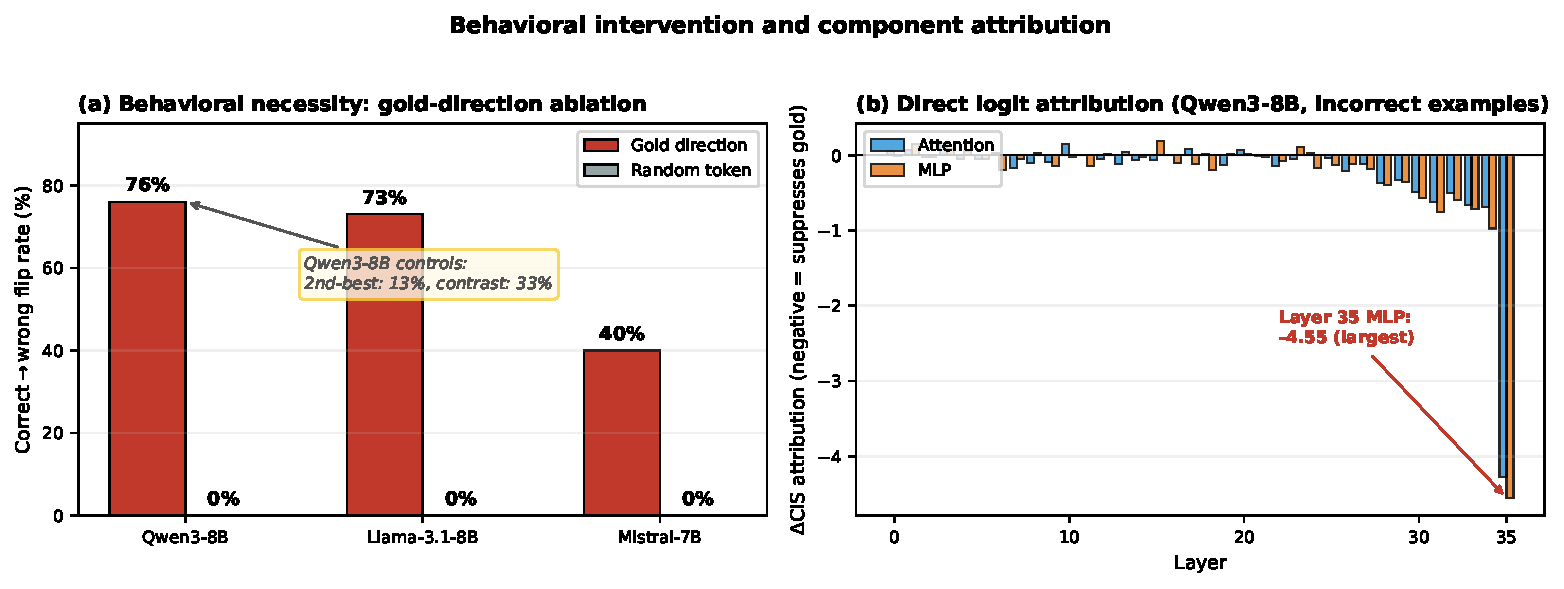
\includegraphics[width=0.95\textwidth]{figures/fig6_intervention.pdf}
\caption{Behavioral intervention and component attribution. (a) Ablating the gold direction flips correct examples to wrong across all model families and scales (77\%, 76\%, 67\%, 87\%, 73\%, 40\% for Qwen3-14B, Qwen3-8B, Qwen3-4B, Qwen2.5-7B, Llama, Mistral), while a random-token control flips almost none. Under a norm-matched protocol, the gold direction flips 83.3\% (8B), 70.0\% (4B), and 75.0\% (14B), versus 38.9\%/35.0\%/55.0\% for second-best, 5.6\%/15.0\%/5.0\% for a random token, and 11.1\%/5.0\%/0.0\% for a Gaussian direction. (b) Component attribution per layer (Qwen3-8B, incorrect examples): the per-layer contribution of attention and the MLP to the margin, with the late-layer MLP (layer 35, $-3.42$) carrying the largest negative direct attribution to the gold-vs-competitor margin.}
\label{fig:intervention}
\end{figure}

\subsection{Calibrated Steering Validates the Taxonomy}

If the formation-versus-preservation distinction captures a real difference in internal state, then a targeted intervention should rescue preservation failures far more than formation failures under the same steering strength. We test this with a calibrated logit bonus: during generation, we add a fixed bonus $\beta$ to the gold token's logit at every decoding step. Because preservation failures have the gold token at final-layer rank $\le5$ in91\% of cases (median rank 1), even a small bonus suffices to tip the gold token to the top prediction and recover the correct answer. Formation failures, by contrast, have the gold token at median rank 23, so the same small bonus cannot bridge the gap.

\begin{table}[t]
\centering
\caption{Calibrated steering recovery rate by failure type. A fixed logit bonus $\beta$ is added to the gold token at every generation step. Preservation failures recover at 4--5$\times$ the rate of formation failures under the same intervention, confirming that the trajectory-based taxonomy identifies differentially repairable errors.}
\label{tab:steering}
\begin{tabular}{lccc}
\toprule
\textbf{Bonus $\beta$} & \textbf{Preservation (n=40)} & \textbf{Formation (n=110)} & \textbf{Ratio} \\
\midrule
1.0 & 2.5\% & 0.9\% & 2.8$\times$ \\
2.0 & 12.5\% & 2.7\% & 4.6$\times$ \\
3.0 & 30.0\% & 6.4\% & 4.7$\times$ \\
5.0 & 32.5\% & 11.8\% & 2.8$\times$ \\
\bottomrule
\end{tabular}
\end{table}

Table~\ref{tab:steering} reports the results. At the bonus that maximizes the recovery-rate ratio ($\beta = 3$), preservation failures recover at 30.0\% while formation failures recover at only 6.4\%, a 4.7$\times$ difference. As the bonus grows larger, both groups recover more, but the gap narrows because a sufficiently large bonus eventually forces any token to the top regardless of its starting rank. The key finding is that at moderate output-logit intervention strengths, the trajectory-predicted preservation failures are substantially more amenable to correction. This validates the taxonomy as differentially repairable: errors diagnosed as preservation failures, where the gold signal once formed, respond far more to late-layer nudging than formation failures where the signal was never established.

We note that this experiment uses the gold token identity and is therefore an oracle proof-of-concept rather than a deployable inference-time method. Its purpose is to validate that the formation-preservation distinction corresponds to a real difference in repairability, not to propose a practical repair system. The sample counts (n=40 preservation, n=110 formation) reflect the natural class proportions among the first 150 error examples evaluated on Qwen3-8B.

\paragraph{Non-oracle closed-loop intervention.}
To demonstrate that the trajectory diagnosis can guide intervention without access to the gold answer, we construct a fully non-oracle pipeline. The steering direction is computed as the mean hidden-state difference between correct and incorrect examples at the last four layers (a standard Representation Engineering contrast; no gold token identity is used). The intervention trigger is the trajectory predictor trained on first-half features. At inference time, we apply activation steering (adding the contrast direction to the final-norm output) only to samples predicted as preservation failures. Under this fully non-oracle pipeline, selective steering achieves 9.1\% recovery per intervention versus 4.0\% for steering all errors indiscriminately, a 127\% efficiency gain while saving 72\% of the intervention budget. The ground-truth breakdown confirms the mechanism: preservation failures recover at 6.6\% while formation failures recover at only 1.8\% (3.7$\times$ difference) under the same non-oracle steering. This demonstrates that the trajectory-based taxonomy provides an actionable, non-oracle trigger for existing intervention methods.

\section{InfoDyn-Bench}

We release \texttt{InfoDyn-Bench}, a benchmark of layered information trajectories for LLM error analysis. Unlike prior resources that store only final-layer outputs or static activations, \texttt{InfoDyn-Bench} records, for each example, the full per-layer trajectory of the gold answer alongside derived failure labels. Table~\ref{tab:benchmark} summarizes its contents. It covers six models across three families and three tasks, and each example carries the raw and tuned-lens trajectories, a set of derived dynamics metrics, a failure-pattern label, and a decay-prediction split.

\begin{table}[t]
\centering
\caption{Contents of \texttt{InfoDyn-Bench}. Each example stores the per-layer trajectory and derived labels; the benchmark is organized so that each downstream use case maps to a stored field.}
\label{tab:benchmark}
\small
\begin{tabular}{lp{8.6cm}}
\toprule
\textbf{Component} & \textbf{Description} \\
\midrule
\textbf{Input} & Question, gold answer, aliases, generated answer, correctness label. \\
\textbf{Trajectory} & Per-layer gold-answer log-probability ($\mathrm{CIS}$), full-vocabulary rank, margin over the competing token, under both the raw and tuned lenses. \\
\textbf{Derived metrics} & Signal-emergence layer (SEL), peak rank, peak $\mathrm{CIS}$, dwell time, peak-to-final decay, sign-change flag, top-5 entry. \\
\textbf{Failure label} & Per-example pattern: \texttt{Absent}, \texttt{Preservation-Failure}, \texttt{Late-Emergent}, \texttt{Decay}, \texttt{Stable}. \\
\textbf{Prediction split} & $t_0$ prefix features, the $y^{\mathrm{decay}}$ label (does the signal decay in the second half?), and final correctness. \\
\textbf{Coverage} & 6 models (Qwen3-4B/8B/14B, Qwen2.5-7B, Llama-3.1-8B, Mistral-7B) $\times$ 3 tasks (TriviaQA, HotpotQA, GSM8K). \\
\bottomrule
\end{tabular}
\end{table}

The benchmark is designed to be used directly by three audiences. First, researchers studying error mechanisms can query the failure labels and per-layer trajectories to test hypotheses about formation versus preservation failures, or to locate the layer at which a gold signal is suppressed (as in Section~\ref{sec:components}). Second, researchers studying decay prediction can use the prediction split to reproduce or extend our decay-prediction and cross-task/cross-model transfer results without re-running the models. Third, researchers building intervention or probing methods can use the derived metrics and labels to select intervention candidates and to measure whether a method changes the failure pattern. Because the trajectories, labels, and splits are stored together and are shared across six models, the benchmark supports the measurement-and-prediction pipeline as a single resource rather than as scattered supplementary files. We include a dataset card with the storage format, licenses, and reproduction scripts.

\section{Discussion and Limitations}

\paragraph{What does "the model knows" mean?}
Competitive decodability is an operational sign of output readiness, not a complete definition of knowledge. We do not equate a top-5 rank with knowledge.

\paragraph{Different failures call for different interventions.}
Formation failures may need retrieval, reasoning correction, or knowledge editing \citep{meng2022rome}. Preservation failures may suit late-layer steering \citep{turner2023activation, zou2023representation}. Reasoning-state failures need tracking intermediate variables. Even though preservation failures are a minority of errors, identifying them is still informative: they are the errors where a correct-answer signal was present at an intermediate layer and subsequently lost, so they are a candidate target for interventions that retain rather than inject knowledge. We leave a causal demonstration of such interventions to future work.

\paragraph{Why do trajectories predict?}
We conjecture that the slope reflects signal stability, the early peak reflects formation speed, and the fluctuation reflects the competitive state. History therefore separates a transient fluctuation from a stable formation better than a single snapshot.

\paragraph{Limitations.}
The margin is an operational proxy, not knowledge itself. Tracking only the final-answer token does not fully describe multi-step reasoning, as in GSM8K. Multi-token answers remain harder to measure. The tuned lens may itself carry probe bias. The competitive-decay taxonomy depends on a competitiveness threshold, although we show the rate changes slowly with that threshold. The gold-direction ablation shows directional specificity under a norm-matched control, but it still does not prove that an information-preservation mechanism is causally responsible for decay, and it does not fully isolate a single causal pathway. Direct logit attribution is not a complete causal mechanism. Our scale analysis covers models from 4B to 14B parameters across three families, but we have not tested very large or reasoning-specialized models, so we do not claim generality beyond this range.

\section{Conclusion}

We showed that the same final error can come from different internal dynamics: a correct-answer signal that never forms, or one that forms and then decays. Naive pairwise logit crossings overstate the second case because of endpoint selection and readout biases. After calibration, a small and task-dependent preservation-failure regime emerges, concentrated in knowledge QA. Calibrated information trajectories identify this regime and give transferable signals for predicting future decay across tasks and model families. We release \texttt{InfoDyn-Bench} to support further study of process-level error diagnosis in language models.

\bibliography{iclr2027_conference}
\bibliographystyle{iclr2027_conference}

\end{document}
